\documentclass[12pt,colorbacktitle,accentcolor=tud1c]{tudexercise}
\usepackage{ngerman}

\usepackage{floatrow}
\usepackage{subfig}
\newfloatcommand{capbtabbox}{table}[][\FBwidth+5cm]
\usepackage{blindtext}
\usepackage{colortbl}
\usepackage{ifthen}

\newcommand{\unit}[1]{{\rm\,#1}}

\title{Space Workshop \newline Dokumentation }
\subtitle{NeXT Generation on Campus}
\subsubtitle{TU Darmstadt}

\newboolean{sensorsDetailed}
\setboolean{sensorsDetailed}{true}


\begin{document}
	\maketitle	
	%\begin{figure}
	%	\newline
	%	\centering
	\bigskip
	\bigskip
	\bigskip
	\bigskip
	\bigskip
	\bigskip
	\begin{figure}[h]
			\centering 
			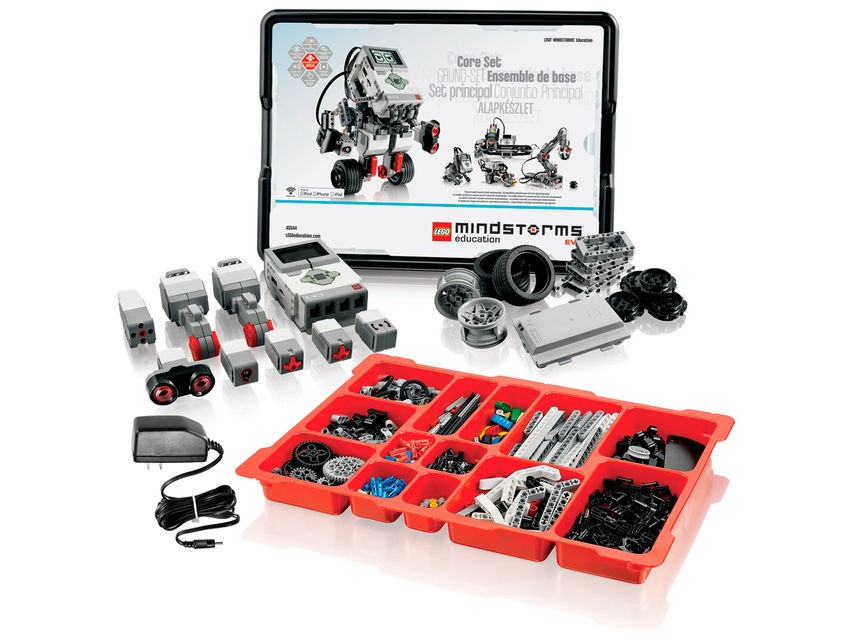
\includegraphics[width=\textwidth]{images/title.jpg}
	\end{figure}
	
	%\begin{center}
	%	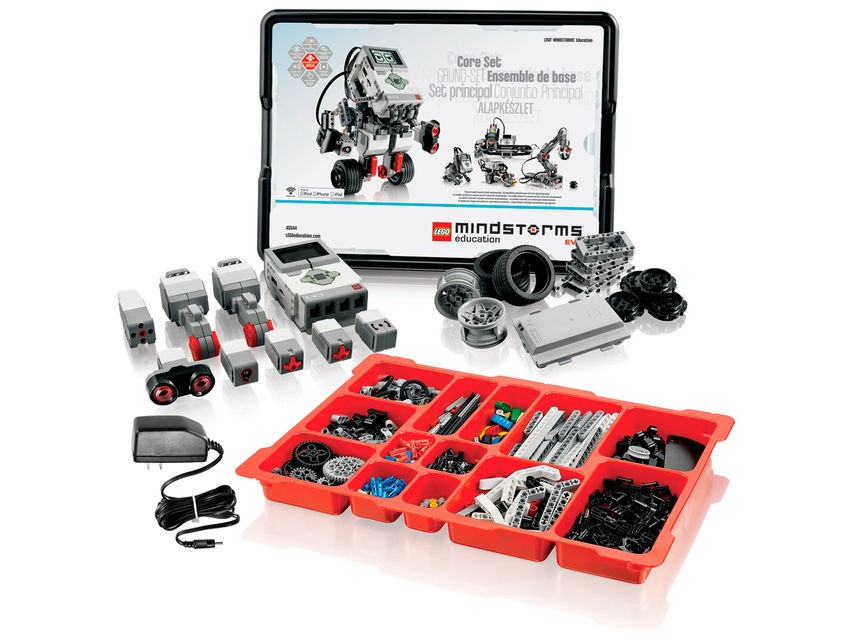
\includegraphics[width=\textwidth]{images/title.jpg}
	%\end{center}
	\newpage
	
	%\end{figure}
	\section{Die EV3-Steuereinheit}
%	\begin{figure}[h]
%		\begin{floatrow}
%			\ffigbox{%
%				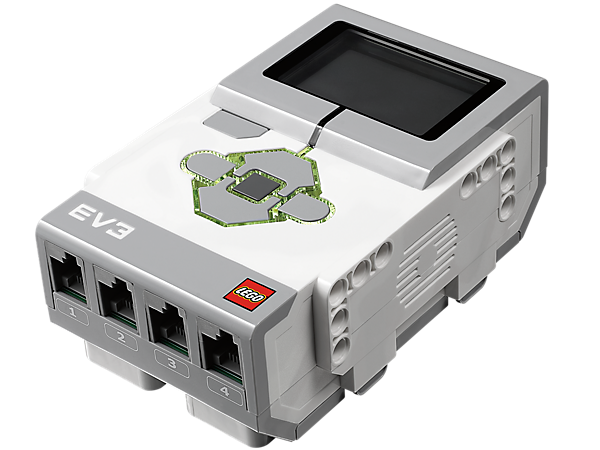
\includegraphics[width=9cm]{images/brick.png}%\rule{3cm}{3cm}%
%			}{%
%				\caption{EV3-Brick}%
%			}
%			\capbtabbox{%
%				\footnotesize
%				\begin{tabular}{|c|c|} \hline
%					Motorausg"ange & MotorPort.A \\
%					&MotorPort.B\\
%					&MotorPort.C\\
%					&MotorPort.D\\ \hline
%					Links & LEFT \\ \hline
%					Rechts & RIGHT \\ \hline
%					Oben & UP \\ \hline
%					Unten & DOWN \\ \hline
%					Mitte & ENTER \\ \hline
%					Oben-Links & ESCAPE \\ \hline
%					Sensoreing"ange & SensorPort.S1 \\
%					&SensorPort.S2\\
%					&SensorPort.S3\\
%					&SensorPort.S4\\ \hline
%				\end{tabular}
%			}{%
%				\caption{Tastenbenennung}%
%			}
%		\end{floatrow}
%	\end{figure}

	
	\begin{figure}[hptb]
		\begin{subfigure}{.65\textwidth}
			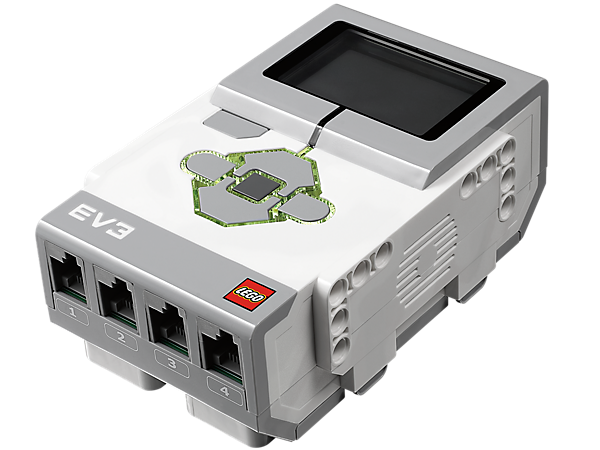
\includegraphics[width=\textwidth]{images/brick.png}
			\\
			\caption{EV3-Brick}
			\label{fig:g1}
		\end{subfigure}%
		\hfill
		\begin{subfigure}{.35\textwidth}
			%\centering
			\begin{tabular}{|c|c|} \hline
				Motorausg"ange & MotorPort.A \\
				&MotorPort.B\\
				&MotorPort.C\\
				&MotorPort.D\\ \hline
				Links & LEFT \\ \hline
				Rechts & RIGHT \\ \hline
				Oben & UP \\ \hline
				Unten & DOWN \\ \hline
				Mitte & ENTER \\ \hline
				Oben-Links & ESCAPE \\ \hline
				Sensoreing"ange & SensorPort.S1 \\
				&SensorPort.S2\\
				&SensorPort.S3\\
				&SensorPort.S4\\ \hline
			\end{tabular}
			\newline  \newline \newline \newline \newline
			\caption{Tastenbenennung}
			\label{fig:g2}
		\end{subfigure}
		%	\caption{Figure caption.}
	\end{figure}
	
	Durch Dr"ucken der mittleren und unteren Taste wird das laufende Programm beendet.
	

		
	\section{Motorsteuerung}
	Dem Roboter stehen 2 starke gro\ss{}e und ein schw"acherer mittelgro\ss{}er Motor zur Verf"ugung.\\ \\
	\begin{figure}[h]
		\begin{floatrow}
			\ffigbox{%
				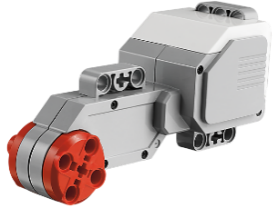
\includegraphics[width=4cm]{images/bigMotor.png}%\rule{3cm}{3cm}%
			}{%
				\caption{gro\ss{}er Motor}%
			}
			\ffigbox{%
				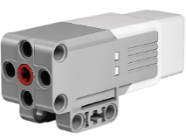
\includegraphics[width=4cm]{images/mediumMotor.png}%\rule{3cm}{3cm}%
				
			}{%
				\caption{mittlerer Motor}%
			}
		\end{floatrow}
	\end{figure}

	
	
	\begin{table}[h]
		\begin{tabular}{|p{0.2\textwidth}| p{0.7\textwidth}|}
			\hline
			Motorausgang & lejos.hardware.port.MotorPort\\ \hline
			gro\ss{}er Motor& lejos.hardware.motor.EV3LargeRegulatedMotor
			 \\ \hline mittlerer Motor & lejos.hardware.motor.EV3LargeMediumRegulatedMotor\\ \hline 
		\end{tabular}
		\caption{ben"otigte Imports}
	\end{table}
 
	\begin{table}[H]
		\begin{tabular}{|p{0.2\textwidth}| p{0.7\textwidth}|}
			\hline
			forward()& Motor dreht sich vorw"arts \\ \hline 
			backward() &  Motor dreht sich r"uckw"arts\\ \hline 
			stop() & Motor stoppt\\ \hline
			rotate(int a) & Motor dreht sich um a Grad\\ \hline
			setSpeed(int x) & setzt die Geschwindigkeit des Motors \\
			& Das Maximum ist hierbei 800\\ \hline
		\end{tabular}
		\caption{wichtige Methoden}
	\end{table}

	Um die Motoren verwenden zu k"onnen, muss zuerst der Motorport und der entsprechende Motor oben in der Datei importiert werden.\\ 
	\textbf{Bsp.: import lejos.hardware.motor.EV3LargeRegulatedMotor;}\\ \\
	Als n"achstes muss 
	Im folgenden Beispiel steht \glqq name\grqq{} f"ur einen frei w"ahlbaren Namen und \glqq X\grqq{} f"ur den Port, also A, B, C oder D.\\
	\textbf{EV3LargeRegulatedMotor name = new EV3LargeRegulatedMotor(MotorPort.X);} \\ 
	\textbf{Bsp.: EV3LargeRegulatedMotor motor = new EV3LargeRegulatedMotor(MotorPort.A);}\\ \\
	Damit sich der Motor bewegt, m"ussen dem Motor nach folgendem Muster eine der gegebenen Methoden gegeben werden.\\
	\textbf{name.Methode;}\\
	\textbf{Bsp.: motor.forward();}

	
	\section{Warten}
	Beim Programmieren ist es immer wieder notwendig, Pausen einzubauen.\\
	Hierf"ur ist der Import \textbf{lejos.utitilty.Delay} notwendig.\\
	Mit der Methode \textbf{Delay.msDelay(int time)} wird eine Pause mit \glqq time \grqq{} Millisekunden ausgef"uhrt. (1000 Milisekunden sind eine Sekunde)\\ \\
	\textbf{Bsp.: Delay.msDelay(2000);}
	
	
	\section{Tasten}
	\begin{table}[h]
		\begin{tabular}{|p{0.2\textwidth}| p{0.7\textwidth}|}
			\hline
			Tasten& lejos.hardware.Button
			\\ \hline 
		\end{tabular}
		\caption{ben"otigter Import}
	\end{table}
	
	\begin{table}[H]
		\begin{tabular}{|p{0.2\textwidth}| p{0.7\textwidth}|}
			\hline
			isDown()& wahr, wenn Taste gedr"uckt \\ \hline 
			isUp() &  wahr, wenn Taste nicht gedr"uckt\\ \hline 
			waitForPress() & wartet, bis Taste gedr"uckt\\ \hline
		\end{tabular}
		\caption{wichtige Methoden}
	\end{table}
Die Methoden werden nach folgendem Muster aufgerufen: \textbf{Button.name.Methode} wobei der \glqq name\grqq{} f"ur die Bezeichnung der Taste steht.\\
\textbf{Bsp.: Button.LEFT.waitForPress();}

Mit der Methode \textbf{\glqq Button.LEDPattern(int i)\grqq{}} wird die LED unter den Tasten gesteuert. Hierbei leuchtet die LED mit unterschiedlichem \textbf{i} von null bis acht in verschiedenen Rhythmen und Farben.

	\section{Lautsprecher}
	\begin{table}[h]
		\begin{tabular}{|p{0.2\textwidth}| p{0.7\textwidth}|}
			\hline
			Lautsprecher& lejos.hardware.Sound
			\\ \hline 
		\end{tabular}
		\caption{ben"otigter Import}
	\end{table}
	
	\begin{table}[H]
		\begin{tabular}{|p{0.2\textwidth}| p{0.7\textwidth}|}
			\hline
			beep()& spielt einen Ton ab \\ \hline 
			twoBeeps() &  spielt den gleichen Ton zweimal ab\\ \hline 
			beepSequence & spielt eine absteigende Tonfolge ab\\ \hline
			beepSequenceUp()& spielt eine aufsteigende Tonfolge ab \\ \hline 
			buzz()& summt \\ \hline 
			setVolume(int vol)& setzt die Lautst"arke auf den Wert vol (0-100) \\ \hline 
		\end{tabular}
		\caption{wichtige Methoden}
	\end{table}
	Die Methoden werden nach folgendem Muster aufgerufen: \textbf{Sound.Methode}\\
	\textbf{Bsp.: Sound.Beep();}

	\section{Display}
	\begin{figure}[h]
		\centering 
		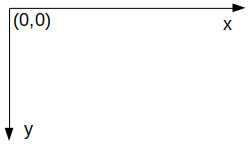
\includegraphics[width=5cm]{images/EV3-CoordSystem.png}
		\caption{Koordinatensystems des Displays}
	\end{figure}
	\begin{table}[h]
		\begin{tabular}{|p{0.2\textwidth}| p{0.7\textwidth}|}
			\hline
			Display& lejos.hardware.lcd.LCD
			\\ \hline 
		\end{tabular}
		\caption{ben"otigter Import}
	\end{table}
	
	\begin{table}[H]
		\begin{tabular}{|p{0.2\textwidth}| p{0.7\textwidth}|}
			\hline
			drawString(String str, int x, int y)& Zeigt einen Text an, beginnend in Spalte x und Zeile y \\ \hline 
			drawInt(int i, int x, int y) &  Zeigt eine Ganzzahl an, beginnend in Spalte x und Zeile y\\ \hline 
			clear() & l"oscht den Inhalt des Displays\\ \hline
			clear(int y)& l"oscht den Inhalt der y-ten Zeile \\ \hline 
			scroll()& verschiebt den Inhalt um eine Zeile nach oben \\ \hline 
		\end{tabular}
		\caption{wichtige Methoden}
	\end{table}

	Das Koordinatensystem auf dem Display hat seinen Ursprung (0,0) oben links und geht in x-Richtung nach rechts 16 Spalten und in y-Richtung nach unten 8 Zeilen. \\ \\
	Das Display wird angesprochen mit: \textbf{LCD.Methode}\\
	\textbf{Bsp.: LCD.drawString(\glqq Hallo Welt!\grqq{}, 0, 0);}

	\ifthenelse{\boolean{sensorsDetailed}}
		{\section{Sensoren}
%\begin{figure}[H]
%	\ffigbox[\textwidth][]{%
%		\begin{subfloatrow}
%			\ffigbox[\FBwidth][]
%			{\caption{Ultraschallsensor}}
%			{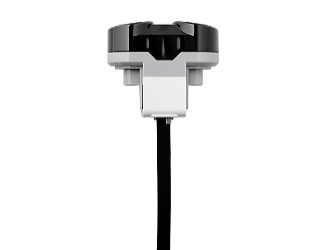
\includegraphics[]{images/ultrasonic.jpg}}
%			\ffigbox[\FBwidth][]
%			{\caption{Farbsensor}}
%			{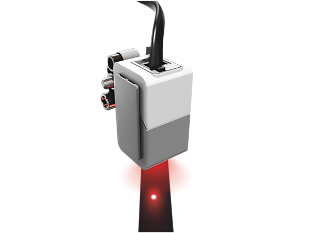
\includegraphics[]{images/color.png}}
%		\end{subfloatrow}%\hspace*{\columnsep}%
%		\begin{subfloatrow}
%			\ffigbox[\FBwidth][]
%			{\caption{Winkelsensor}}
%			{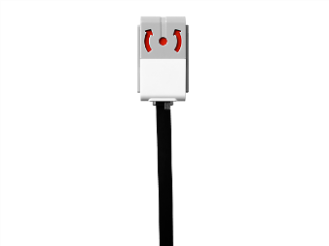
\includegraphics[]{images/gyro.png}}
%			\ffigbox[\FBwidth][]
%			{\caption{Ber"uhrungssensor}}
%			{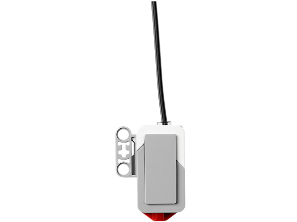
\includegraphics[]{images/touch.png}}
%		\end{subfloatrow}
%	}{}
%\end{figure}

\begin{figure}[hptb]
	\begin{subfigure}{.225\textwidth}
		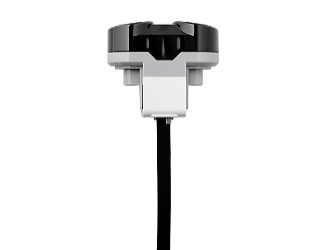
\includegraphics[width=\textwidth]{images/ultrasonic.jpg}
		\\
		\caption{Ultraschallsensor}
		\label{fig:g1}
	\end{subfigure}%
	\hfill
	\begin{subfigure}{.225\textwidth}
		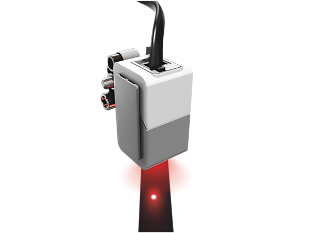
\includegraphics[width=\textwidth]{images/color.png}
		\\
		\caption{Farbsensor}
		\label{fig:g2}
	\end{subfigure}
	\hfill
	\begin{subfigure}{.225\textwidth}
		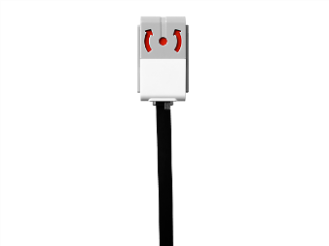
\includegraphics[width=\textwidth]{images/gyro.png}
		\\
		\caption{Winkelsensor}
		\label{fig:g2}
	\end{subfigure}
	\hfill
	\begin{subfigure}{.225\textwidth}
		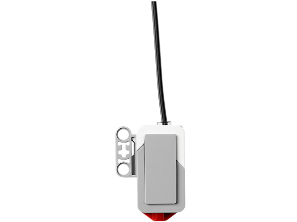
\includegraphics[width=\textwidth]{images/touch.png}
		\\
		\caption{Ber"uhrungssensor}
		\label{fig:g2}
	\end{subfigure}
%	\caption{Figure caption.}
\end{figure}

\begin{table}[h]
	\begin{tabular}{|p{0.2\textwidth}| p{0.7\textwidth}|}
		\hline
		Sensorausgang & lejos.hardware.port.SensorPort\\ \hline
		Ultraschallsensor& lejos.hardware.sensor.EV3UltrasonicSensor
		\\ \hline 
		Farbsensor & lejos.hardware.sensor.EV3ColorSensor\\ \hline 
		Winkelsensor & lejos.hardware.sensor.EV3GyroSensor\\ \hline 
		Ber"uhrungssensor & lejos.hardware.sensor.EV3TouchSensor\\ \hline 
	\end{tabular}
	\caption{ben"otigte Imports}
\end{table}

\begin{table}[H]
	\begin{tabular}{|p{0.2\textwidth}| p{0.7\textwidth}|}
		\hline
		setCurrentMode\newline (String mode)& setzt den Modus des Sensors \\ \hline 
		sampleSize() &  gibt die Anzahl der zur"uckgegeben Werte zurück\\ \hline 
		fetchsample(float[] signal, int offset) & Sensor misst und speichert es im Array \textbf{signal} ab Stelle \textbf{offset}\\ \hline
		getColorID() &  Farbsensor gibt erkannte Farbe zur"uck (-1=keine Farbe, 0=Rot, 1=Gr"un, 2=Blau, 3=Gelb, 6=Wei\ss{}, 7=Schwarz, 13=Braun)\\ \hline 
	\end{tabular}
	\caption{wichtige Methoden}
\end{table}

\begin{table}[H]
	\begin{tabular}{|p{0.2\textwidth}| p{0.7\textwidth}|}
		\hline
		Ultraschallsensor& Distance (Sensor gibt Distanz in Metern zur"uck) \\ \hline 
		Farbsensor &  Ambient (Sensor gibt Umgebungshelligkeit in Werten zwischen 0 und 1 zur"uck)\\ \hline 
		Winkelsensor& (Sensor gibt Winkel zur"uck)\\ \hline
		Ber"uhrungssensor& (Sensor gibt zur"uck, ob Taste gedr"uckt (1) oder nicht gedr"uckt (0) ist)\\ \hline
	\end{tabular}
	\caption{Modi}
\end{table}

Die Benutzung der Sensoren ist auf den ersten Blick etwas kompliziert, jedoch folgt die Benutzung einem festen Aufbau.\\

Zuerst muss wie bei den Motoren der Sensor benannt werden.\newline
\textbf{Bsp.: EV3UltrasonicSensor ultra = new EV3UltrasonicSensor(SensorPort.S1)}\\ \\
Als n"achstes muss der Sensor in den richtigen Modus gesetzt werden mit \newline \textbf{sensorname.setCurrentMode(String mode)}\\
\textbf{Bsp.: ultra.setCurrentMode(\glqq Distance\grqq{});}
\\ \\
Der n"achste Schritt ist das Anlegen eines Arrays, in dem die Daten gespeichert werden. Hierbei wird direkt mit \textbf{sampleSize()} die Gr"o\ss{}e gesetzt.
\textbf{Bsp.: float[] signal = new float[sensorname.sampleSize()];}
\\ \\
Um neue Daten zu erfassen wird mit dem Sensor die Methode \textbf{fetchSample} aufgerufen und im vorher angelegten Array gespeichert.\\
\textbf{Bsp.: ultra.fetchSample(signal, 0);}

}
		{\section{Sensoren}
\newpage}
	\section{Kurze "Ubersicht "uber Java}
	\arrayrulecolor{white}
	\begin{table}[h]
		\renewcommand{\arraystretch}{1.5}
		\begin{center}
			\begin{tabular}{|p{0.3\textwidth}|p{0.7\textwidth}|}
				\hline
				Schleife mit Bedingung& while(Bedingung) \{Programmcode\} \tabularnewline
				\space & \scriptsize Beispiel: while(i<100)\{...\} \tabularnewline
				\hline
				Z"ahlschleife& for(Start; Bedingung; Z"ahlschritte) \{Programmcode\} \tabularnewline
				\space & \scriptsize Beispiel: for(int i=0;i<10;i++)\{...\} \tabularnewline
				\hline
				Bedingung& if(Bedingung) \tabularnewline
				\space& \{wenn die Bedingung wahr ist, wird dieser Code ausgef"uhrt\} \tabularnewline
				\space & else \tabularnewline
				\space & \{wenn die Bedingung falsch ist, wird dieser Code ausgef"uhrt\}
				\tabularnewline
				\hline			
			\end{tabular}
		\end{center}
	\end{table}
	
	\section{Quellen}
	Die Dokumentation mit weiteren Methoden befindet sich unter:\\
	lejos.org/ev3/docs/\\ \\
	
	Die Lejos Software kann auf der folgenden Seite heruntergeladen werden. Weiterhin gibt es dort ausf"uhrliche Anleitungen zum Einrichten auf dem EV3-Roboter:\\
	lejos.sourceforge.io\\ \\
	
	Der genutzte Java-Editor ist kostenfrei im Netz verf"ugbar:\\
	javaeditor.org\\ \\
	
	Bei Fragen stehen wir immer gerne zur Verf"ugung:\\
	next-generation@etit.tu-darmstadt.de \\ \\
	
	Die Bilder sind der Internetseite des offiziellen Lego-Onlineshops lego.com entnommen. Die Urheberrechte befinden sich im Besitz der LEGO Gruppe, diese Anleitung ist unabh"angig und wurde von der LEGO Gruppe weder autorisiert noch gesponsert.
  
   
    
\end{document}
